% todo: 
% expansion -> initial capacity and load factor instead of 0.7?

\chapter{NVM-enabled hashmap}
In this chapter we will discuss the key component of our system which allows us to reliably manage data locally using the non-volatile memory. 

% \noindent \tk{General remarks: 
% \begin{itemize}
    % \item the section looks much better!
    % \item when I add a remark, rarely adding one short sentence to the text is enough ;)
    % \item always ensure that a sentence has a purpose: either it gives some
    % important information, or joins two bodies of text together and thus cannot be omitted, 
    % \item consider putting listings in figures, so you can control
    % where they appear in the text,
    % \item ensure you have a consistent naming convention: locks, mutexes, small hashmaps, segments, cells of arrays of segments, item, entry, etc.
    % \item consider simplifying the used names of class fields so they are simpler but still meaningful; \locks could be simply \texttt{mutexes} (see also my comment about mutexes vs readers-writer locks); \texttt{caulculateIndex()} and \texttt{calculateIndex2()} are \textbf{not} good method names
% \end{itemize}}
    % \tk{if it's a name, don't use the; so e.g., \texttt{foo()} encapsulates some logic or the \texttt{foo()} function encapsulates some logic; it has to be fixed in several places}


\section{Assumptions}

    % \tk{Maybe something like this: In the intro, when you describe DHT, you will need to explain what a hash table (or hash map) is, so a datastructure which functions as an associative array containing pairs of keys and values. In order to facilitate fast entry lookup, entries in the hash map are group based on .... Then here you can say something like this: Each replica of $<$name of your system$>$ stores data locally in a \emph{generic} hash map, which means that ... In order to calculate the hash for a key ... We can use standard hashing functions for basic types such as ... However, to use the hash map with non-standard/user-defined/... data types ...}

    In order to describe the \DHT system, it is best to get acquainted with a hashmap itself at first. 
    It is an associative array containing pairs of keys and values.
    In order to facilitate fast entry lookup, entries in the hash map are based on keys. 
    They are unique for each element and enable its unambiguous identification. 
    The elements position in the structure is defined by a hash value of the element key. 
    
    Each replica of \DHT stores data locally in a \emph{generic} hash map.
    The data structure is able to store any type of keys and values, what requires the use of a generic hashing function. 
    We can use a standard method from the \std namespace for basic types such as \texttt{int} or \texttt{string}. 
    However, to use the hash map with non-standard data types, the programmer needs to define the hashing function himself.
    
    Since the \libpmemobj library does not support polymorphic types, it was not possible to use the map interface from the \std namespace. 
    It had to be implemented from the ground up.
    Therefore, the hashmap interface defines methods similarly to the \HashMap in Java \cite{HashMapJava}. It provides basic operations such as: \insertMethod, \getMethod or \removeMethod and an \Iterator object. 
    
    In order to ensure high performance of modern multicore CPU architecture, it is implemented in a way enabling concurrent access. 
    Multiple threads working at the same time should not imply incorrect data or tardiness. 
    The provided solution is to compose the \NvmHashMap of several \internalHashMaps with the ability to expand.
    It is analogous to the \ConcurrentHashMap in Java 7 \cite{ConcurrentHashMapJava} and covered in the next section.
    
    % \tk{Do NVM impose anything? Because you use NVM, you approach certain aspects of the design and implementation differently, e.g. ...}
    In addition, using non-volatile memory requires different approach to certain aspects of design and implementation.
    Particular attention should to be paid to the crash consistency support. 
    Scenarios such as power failures or application crashes need to be considered.
    
\section{Overview}

    The listing \ref{NvmHashMap} presents the \NvmHashMap interface. 
    \texttt{K} represents the generic type of key and \texttt{V} the generic type of value. 
    % The \texttt{internalHashMapIndex} stands for the array that is expanding
    % \tk{You haven't mentioned any array yet nor anything about expansion. See my earlier comments.}.
    
\begin{figure}[ht] 
\renewcommand{\figurename}{Listing}
    \begin{lstlisting}
class NvmHashMap {
    int loadFactor;
    unsigned long long int hash(K key);
    V insert (K key, V value);
    V get (K key);
    V remove (K key);
    void expand (int internalHashMapIndex);
    
    friend class Iterator<K,V>;
}
    \end{lstlisting}
\label{NvmHashMap}
\caption{\NvmHashMap interface}
\end{figure}
    In order to solve the concurrency issue, the hashmap implementation is based on the \ConcurrentHashMap from the seventh version of Java \cite{ConcurrentHashMapJava}. 
    This class consists of sixteen smaller hashtables with individual locks on each of them which separates different segments for the threads to work on.
    \NvmHashMap is constructed in a similar way, having a specified number of \internalHashMaps with separate locks per each.
    The number may increase while inserting elements to the structure depending on the \texttt{loadFactor}.
    Furthermore, the \ConcurrentHashMap \textit{supports full concurrency of retrievals and adjustable expected concurrency for updates} \cite{ConcurrentHashMapJava}. 
    The hashmap presented in this thesis follows this approach with the writers-readers lock.
    
    Considering the NVM support, all write operations need to be carried out in transactions. 
    If a transaction fails between tasks for example due to power outage, it will be automatically rollbacked.
    This way the data stays consistent even in the event of possible system failures.
    % \tk{When you say something, explain it if its not obvious. This is not obvious at all. What can go wrong if there were no transactions?}

\section{Implementation}

    \subsection{Generic hashmaps} 
        Since the \NvmHashMap is generic, we need to be able to calculate the hash value of keys of arbitrary types. 
        To this end, we use a hash method from the \std namespace. 
        Once the hash is calculated, we store it as an \texttt{unsigned long long} integer.
        At the end the function returns an absolute value of the hashed key.
        
        Using the basic types from the \std namespace in the \NvmHashMap is quite effortless.
        However, it requires additional work when it comes to client-defined key types.
        The programmer needs to overload the comparison operator which is used for operations such as \insertMethod, \getMethod or \removeMethod.
        He must also provide a hash functor.
        We demonstrate how it can be accomplished by using a template inside the \std in the Listing \ref{StdHashOverload} below.
            
\begin{figure}[ht]
\renewcommand{\figurename}{Listing}
\begin{lstlisting}
struct newStructure {
    int firstAttribute;
    std::string secondAttribute;
    
    bool operator==(const newStruct &element) const {
        return (firstAttribute == other.firstAttribute 
            && secondAttribute == other.secondAttribute);
    }
};

namespace std {
    template <>
    struct hash<newStructure>
    {
        std::size_t operator()(const newStructure &element) const
        {
            using std::hash;
            using std::string;

            return ((std::hash<string>()(element.firstAttribute) << 5)
                ^ (std::hash<int>()(element.secondAttribute) << 1);
        }
    };
}
\end{lstlisting}
\caption{User-defined key usage in the \NvmHashMap}
\label{StdHashOverload}
\end{figure}

    \subsection{Structure}

        As mentioned before, \NvmHashMap consists of an array of smaller hashtables which are called \internalHashMaps.
        % \tk{this name is somewhat cumbersome, maybe you can think of something better?}. 
        The use of an array allows us to split the work in an even way between threads. 
        It lowers the probability of multiple threads waiting on the same critical section.
        The number of the smaller hashmaps is kept separately in a parameter named \internalMapsCount. 
        Its value should be correlated with the number of threads, is provided by the programmer and rounded down to the previous power of two.
        If not specified, it is set to 8 by default. 
        To support inter-thread synchronisation, one more array is maintained, which is called \locks and will be discussed later.

\begin{figure}[ht]
\renewcommand{\figurename}{Listing}
\begin{lstlisting}
class internalHashMap {
    pmem::obj::persistent_ptr<Segment<K, V>[]> segments;
    pmem::obj::p<int> arraySize;
    pmem::obj::p<int> elementsCount;
}
\end{lstlisting}
\caption{\internalHashMap interface}
\label{internalHashMap}
\end{figure}

        The \internalHashMap interface is presented in Listing \ref{internalHashMap}. 
        The class contains an array of lists which are called \Segments and store the entries.
        % \tk{what is stored there?}
        The \texttt{segmentsCount} stands for the number of lists. 
        It is set to 16 initially and may be increased by expansion as the data is inserted into \NvmHashMap. 
        The last member of the class is named \texttt{elementsCount}. 
        It is set to 0 at first and is used to track how many elements are in all \Segments in \internalHashMap. 
        We use the value of this field to decide whether it is a proper time to execute an \expandMethod.
        
\begin{figure}[ht]
\renewcommand{\figurename}{Listing}
\begin{lstlisting}
class Segment {
    pmem::obj::persistent_ptr <SegmentObject<K, V>> head = nullptr;
    pmem::obj::p<int> hash;
    pmem::obj::p<int> size = 0;
}
\end{lstlisting}
\caption{Segment interface}
\label{Segment}
\end{figure}

        The \Segment class is used for storing the data entries in a linked list which is supported out of the box by the \libpmemobj library.
        The class is composed of a persistent pointer to the head of the list, its size and a hash value corresponding to all the elements.
        The entries are called \texttt{SegmentObjects}. 
        Each one consist of a key and value of any type along with a persistent pointer to the next element. 
        
        % \tk{What is it for? Say it's a linked list, and that as such is supported out of the box by the library; this discussion maybe should be in the assumption - you decided to implement the hashmap in this fashion because certain abstractions are already available.}
        
    \subsection{Concurrency} 
    
        % \tk{General remark first: you use locks to synchronize accesses to the hashmap. More precisely, you use an array of ... (stored in ...). Each element of the array is... BTW, isn't a mutex by definition a mechanism that guarantees only mutual exclusion (so there is no shared-access mode for read-only operations? Maybe consider a different name.}
        
        The data integrity during concurrent access is provided by using locks. 
        More precisely, we use a \locks array stored in the \NvmHashMap class.
        Each element of the array is responsible for another cell in the \internalHashMap.
        That way if a thread is performing an operation, only the \internalHashMap to which the item belongs is locked instead of the entire \NvmHashMap. 
        This allows the threads working on different sections to concurrently access different sections of the \NvmHashMap.  
        
        Operations that require exclusive access to the \internalHashMap are \insertMethod, \removeMethod and \expandMethod.
        They use \texttt{unique\_locks} \cite{UniqueLock} from the \std name space.
        It means that when one thread performs a write operation, no other thread has access to the hash map, neither to write or read an element. 
        On the contrary, the \getMethod or \iterateMethod methods do not require exclusive access to the map. 
        They are both read operations and do not change any data, therefore can be performed concurrently.
        The only used lock is an \std \texttt{shared\_lock} \cite{SharedLock} which allows the others to read data at the same time. 
        This solution is the so called \textit{readers-writers lock}. 
        % \tk{What is a shared mutex? In the pseudocodes, where you do the unlock operations? Moreover, you seem to aquire the locks in the same fashion for both write and read operations. 0.7 should be a define. There are some parenthesis missing in listing 3.5.}
        
    \subsection{Automatic hashmap expansion}
        % \tk{This sentence is not necessary.} One of the assumptions made for the discussed structure was an automatic extension \tk{extension does not mean the same thing as expansion!} of the \internalHashMap. 
        The \expandMethod method is performed while inserting an element on a certain condition.
        In order for the \internalHashMap to resize, the \texttt{elementsCount} has to exceed the product of the \texttt{loadFactor} and the \texttt{arraySize}.
        %\tk{I guess it's not the way it is typically done. See \url{https://stackoverflow.com/questions/23029161/what-will-be-if-put-in-hashmap-more-than-capacity}}
        That requirement is checked only for the \internalHashMap to which an element is being added. 
        Once that condition is met, the program allocates memory for the new \internalHashMap with 4 times bigger size. 
        Then it iterates through the old \internalHashMap in order to insert all previously added elements to the new one. 
        It uses for this purpose \texttt{insertIntoInternalHashMap} method, the exactly same one as in inserting.
        This way all items have a newly calculated hash after resizing and therefore are evenly distributed in the array. 
        As mentioned previously, the expansion procedure requires an exclusive access to the \internalHashMap. 
        Therefore it takes place after locking the small hashmap for insertion in an exclusive mode.

    \subsection{Implementation of the hashmap methods}
        As previously stated, the hashmap supports \insertMethod, \getMethod and \removeMethod operations, as well as an \Iterator class which allows us to iterate over the whole \NvmHashMap.
        Any kind of item operation requires two indexes to be calculated. 
        The first one, \texttt{chooseInternalHashMap}, indicates the \internalHashMap corresponding to the current thread and the second one, \texttt{chooseSegment}, marks the right \Segment in the \internalHashMap. 
        They are both computed by hashing the key and performing bit operations to calculate the offset.
    
\begin{figure}[ht]
\renewcommand{\figurename}{Listing}
\begin{lstlisting}
V insert (K key, V value) {
    int hashMapIndex = chooseInternalHashMap();
    lock(locks[hashMapIndex]);
    if (internalHashMap[hashMapIndex].elementsCount > 
            0.7 * internalHashMap[hashMapIndex].arraySize) {
        expand(hashMapIndex);
    }
    int result = insertIntoInternalHashMap(key, value, internalHashMap[hashMapIndex]);
    internalHashMap[hashMapIndex].elementsCount += result;
    unlock(locks[hashMapIndex]);
}
    
int insertIntoInternalHashMap(K key, V value, internalHashMap<K, V> &aos) {
    int index2 = chooseSegment();
    persistent_ptr element = aos.segments[segmentIndex].head;
    while (element->next) {
        if (element.key == key) {
            updateElement(V value);
            return 1;
        } 
        element = element -> next;
    }
    appendToTheEnd(V value);
    return 1;
}
\end{lstlisting}
\renewcommand{\figurename}{Listing}
\caption{\insertMethod method}
\label{insertMethod}
\end{figure}
        The \insertMethod method (whose pseudocode we give in Listing \ref{insertMethod}) works as follows.
        Firstly, we calculate the first index to determine the \internalHashMap to work on.  
        Once the map on which work should be performed is known, the program locks access to the corresponding \internalHashMap. 
        Before inserting it is checked whether the expand function should be executed. 
        If not, it is proceeded straight to inserting the item into the \internalHashMap. 
        The next thing is to compute the Segment index and to iterate through the list. 
        If it finds an element with the same key on the list, it updates it with a current value, otherwise appends it to the end.
        Once the addition was successful, it increments the \texttt{elementsCount} by one. 
        The important thing is to carry out all these operations in a transaction. 
        This way if there is some failure while adding an element, the size will not be increased. 
        By doing this the consistency of the hashmap is provided.
        % \tk{In the pseudocodes -- \emph{Did not found} what?}
        
\begin{figure}[ht]
\renewcommand{\figurename}{Listing}
\begin{lstlisting}
V get (K key) {
    int hashMapIndex = chooseInternalHashMap();
    int segmentIndex = chooseSegment();
    lock_shared(locks[index];
    persistent_ptr element = internalHashMap[hashMapIndex].
                                    segments[segmentIndex].head;
    while (element->next) {
        if (element.key == key) {
            return element;
        }
        element = element -> next;
    }
    unlock_shared(locks[hashMapIndex]);
    throw "Did not found element" exception
}
\end{lstlisting}
\caption{\getMethod method}
\label{getMethod}
\end{figure}

        The pseudocode for the \getMethod method is provided in Listing \ref{getMethod}. 
        To get an item, at first the two indexes are computed. 
        Once they are both known, a a matching \internalHashMap is locked but in this case as a \texttt{unique\_lock} \cite{UniqueLock} from the \std namespace.
        Then the function begins to iterate over the list. 
        Once the item is found, it simply returns its value, otherwise an exception is thrown.
        
\begin{figure}[ht]
\renewcommand{\figurename}{Listing}
\begin{lstlisting}
V remove (K key) {
    int index = chooseInternalHashMap();
    int index2 = chooseSegment();
    lock(locks[hashMapIndex]);
    persistent_ptr element = internalHashMap[hashMapIndex].segments[segmentIndex].head;
    while (element->next) {
        if (element.key == key) {
            removeElement();
            internalHashMap[hashMapIndex].segments[index2].size -= 1;
            internalHashMap[hashMapIndex].elementsCount -= 1;
            return value;
        }
        element = element -> next;
    } 
    unlock(locks[index]);
    throw "Did not found element" exception
}
\end{lstlisting}
\caption{\removeMethod method}
\label{removeMethod}
\end{figure}

        The \removeMethod function introduced in the Listing \ref{removeMethod} is quite similar to the \getMethod one. 
        In the beginning, the two indexes are calculated. 
        Then, again a corresponding \internalHashMap is locked in a shared mode (\texttt{unique\_lock} \cite{UniqueLock}).
        The programs starts to iterate over the segment and when the item is found, it opens a transaction. 
        It deletes the element from the list and decreases corresponding sizes by 1.
        If the element is not found, the program throws an exception.

        The \NvmHashMap implements also an \Iterator which can be used to easily iterate through the hashmap.
        After initialization, it locks the first cell of the \internalHashMap and sets a pointer to the head of the list.
        It provides a boolean method called \texttt{next} which moves the pointer to the next object of the list until its end. 
        While accessing every element the method locks the corresponding shared lock again. 
        When it finishes iterating over the list, it moves to the next \Segment and locks the \internalHashMaps once more. 
        Once all the segments are iterated over, the function repeats the same steps for the next \internalHashMap until there are no left to loop over.
        
        It is worth noting that ensuring a correct iteration over a concurrent data structure such as the \NvmHashMap is not easy. 
        Since the \iterateMethod method uses only a shared lock, it may provide slightly inconsistent image of the hashmap while working in a multithreaded mode.
        If one thread starts iterating and another one removes an item afterwards, the first one may still see it in a hashmap. 
        The same way, if one adds an element, it may not be visible for the second one yet. 
        This inconsistency could have been solved using an exclusive mode of locking, however, it would reduce the availability of data. 
        Since it is extremely difficult to achieve both consistency and high availability at the same time, it has been agreed to focus on the accessibility.

\section{Evaluation}

    \subsection{Correctness tests}
        In order to ensure that the hashtable works correctly, we developed a range of unit tests.
        To this end we used the \GoogleTest library \cite{GoogleTest}.
        The unit tests verify the correctness of the implemented operations: \insertMethod, \getMethod, \removeMethod and \iterateMethod. 
        They are performed on two different instances of the hashtable: \integersMap and \stringsMap.
    
        % \tk{You need to say first that that you have several tests}
        There are several tests performed.
        The first test works in single-threaded mode and inserts a number of elements with a known sum.
        Then it iterates through the hashmap ans sums the elements up.
        At the end an assert checks whether the two values are equal.
        The test is run on both \NvmHashMap instances but in the \stringsMap one integers are cast to strings.
        
        The next tests focus on insert, get and remove functions. 
        We run them both in the single and the multithreaded mode (using 8 threads). 
        Each thread inserts 100000 elements. 
        Then, one test case retrieves the previously added values while the other test tries to remove them.
        In order for the test to pass, all inserted items need to be either found or deleted.
        Considering the fact that both get and remove methods return a value of an element identified by a key, for each case the received value is compared with the added one using an assert.
        
        % \tk{What you're probably trying to explain here is that each test is really a separate program instance. In traditional systems when the program ends, the data kept in memory is lost, but here you need to do some garbage collecting, right?}
        One of issues that needs to be taken into account while developing unit tests is the non-volatile nature of the data kept in the \NvmHashMap. 
        In a traditional system which uses RAM memory, many tests can be performed in one test suite as the data kept in memory is automatically freed in between by a garbage collector.
        However, the presented system keeps the data in the non-volatile memory even after the test finishes.
        Therefore if two tests are executed one after another and the inserting functionality is the main purpose of the second test case, it may not be clear whether the program works properly or it refers to the previous values. 
        Since the tests job is to detect if the code works correctly, implemented functions cannot be relied to delete all values before next test. 
        The chosen solution is to run each each test as separate program instances.
        That way the files can be deleted and the memory cleared in between tests.

    \subsection{Performance tests}
        The performance tests aim at comparing the effectiveness of the NVM-enabled hashtable with the \unorderedMap from the \std name space \cite{UnorderedMapCpp}. 
        The \unorderedMap is an associative structure that contains pairs of keys and values identified by the keys. 
        The elements are organised into buckets depending on their hash value. 
        The interface provides methods such as \texttt{insert}, \texttt{find} and \texttt{erase} which are analogous to the methods from the \NvmHashMap and are the subject to the following tests.
        
        The tests measure the time it takes to insert, get and remove 125000 elements. 
        The number of items is limited by the memory size. 
        We conducted tests for respectively 1, 2, 4, 8 and 16 threads on the following computer environment:
        \begin{itemize}
            \item Processor IntelCore i5-4210U 
            \item Numer of cores: 2
            \item Processor frequency: 1.7 GHz -- 2.7 GHz
            \item NVM emulation: 2 GB, RAM: 6 GB
            
        \end{itemize}
        
\begin{figure}[ht]
    \centering
    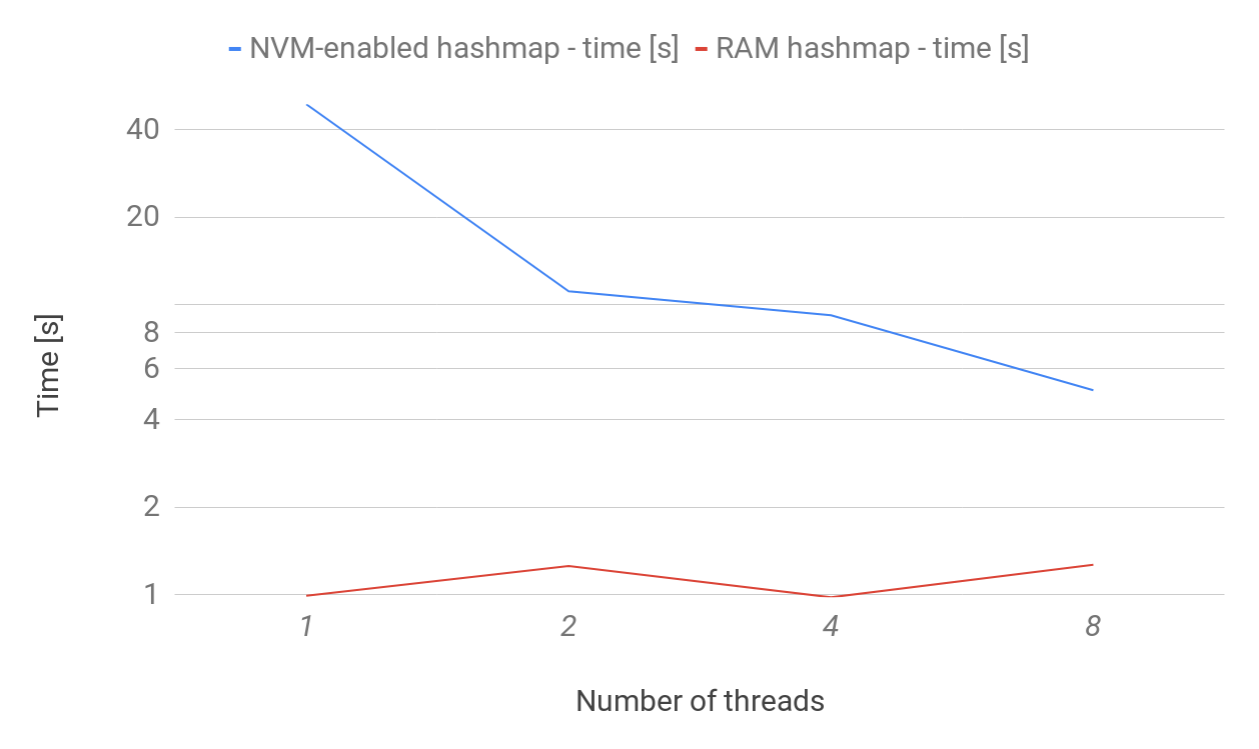
\includegraphics[width=0.8\textwidth]{thesis/figures/insert.png}
    \caption{Time measurements for \insertMethod operation comparing the NVM-enabled hashtable with unordered map}
    \label{insertPlot}
\end{figure}

\begin{figure}[ht]
    \centering
    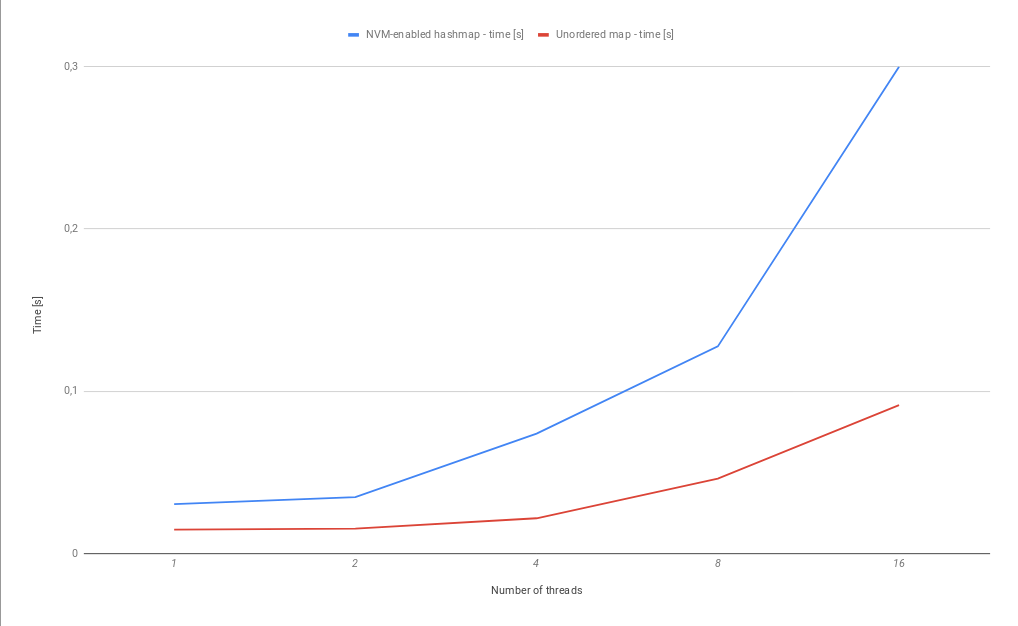
\includegraphics[width=0.8\textwidth]{thesis/figures/get.png}
    \caption{Time measurements for \getMethod operation comparing the NVM-enabled hashtable with unordered map}
    \label{getPlot}
\end{figure}

\begin{figure}[ht]
    \centering
    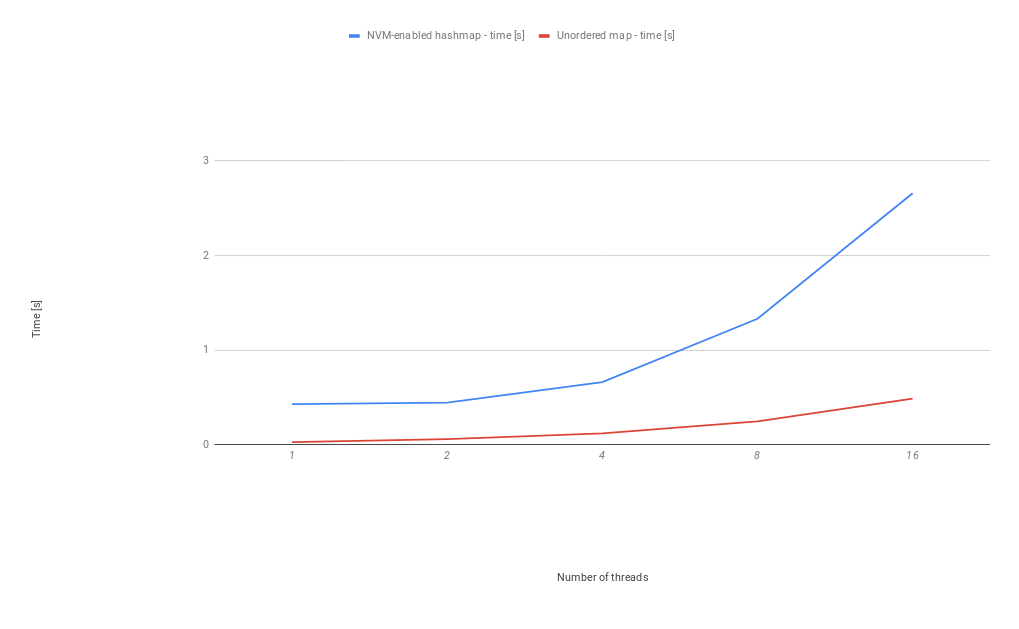
\includegraphics[width=0.8\textwidth]{thesis/figures/remove.png}
    \caption{Time measurements for \removeMethod operation comparing the NVM-enabled hashtable with unordered map}
    \label{removePlot}
\end{figure}

        The tests results are shown on plots \ref{insertPlot}, \ref{getPlot} and \ref{removePlot}. 
        There is a noticeable NVM-induced time overhead. 
        Both \insertMethod and \removeMethod operations turn out to be about five times slower using NVM than RAM. 
        The \getMethod method is about three times slower in the \NvmHashMap.
        All methods take more time as the number of threads increases, as a natural consequence of using locks.
        
        % \tk{You need to say how big is the difference, what are the trends, does your system scale with the increasing number of threads}
        
        The \insertMethod operation takes the longest time since it allocates memory and creates a new object.
        It is about five times slower than
        Furthermore, it requires an exclusive access to the \internalHashMap and executes an expansion when needed. 
        The \removeMethod method is a bit faster than the NVM \insertMethod. 
        However, the noticeable tardiness compared to the \unorderedMap is caused by a transaction destroying a persistent object and an exclusive lock on the internal map.
        The \getMethod method is the fastest one. 
        It locks the \internalHashMap in a shared mode only and does not modify any of the data. 
        
        To sum up, the \NvmHashMap is slower compared to the \unorderedMap. 
        The observed overhead is an effect of the NVM support, since it requires running transactions and operating on persistent objects. 
        The non-volatile memory is emulated on DRAM and includes handling file operations which also causes delays.
        Nevertheless it is worth noticing that provided system is scalable.
        
\section{Conclusions}
    The chapter covered the \NvmHashMap, a hash table which supports non-volatile memory. Implementing the described system has involved a number of challenges, such as support for generic types and concurrency or choosing the suitable hash function. 
    % \tk{This kind of sentence probably should be in the final conclusions.} However, using the \libpmemobj library has helped us to understand better how NVM works. 
    
    Executing performance tests has allowed us to evaluate the effectiveness of the implemented data structure. 
    As the tests show, there are some inherent costs of enabling the non-volatile memory. 
    Unsurprisingly, the \NvmHashMap turns out to be slower by about four times than a hash map which uses traditional RAM. % \tk{by how much?}
    Moreover, while developing an NVM-enabled system more emphasis should be put on the consistency due to the persistent character of the data.